\documentclass[twoside]{book}

% Packages required by doxygen
\usepackage{fixltx2e}
\usepackage{calc}
\usepackage{doxygen}
\usepackage[export]{adjustbox} % also loads graphicx
\usepackage{graphicx}
\usepackage[utf8]{inputenc}
\usepackage{makeidx}
\usepackage{multicol}
\usepackage{multirow}
\PassOptionsToPackage{warn}{textcomp}
\usepackage{textcomp}
\usepackage[nointegrals]{wasysym}
\usepackage[table]{xcolor}

% NLS support packages
\usepackage[spanish]{babel}
% Font selection
\usepackage[T1]{fontenc}
\usepackage[scaled=.90]{helvet}
\usepackage{courier}
\usepackage{amssymb}
\usepackage{sectsty}
\renewcommand{\familydefault}{\sfdefault}
\allsectionsfont{%
  \fontseries{bc}\selectfont%
  \color{darkgray}%
}
\renewcommand{\DoxyLabelFont}{%
  \fontseries{bc}\selectfont%
  \color{darkgray}%
}
\newcommand{\+}{\discretionary{\mbox{\scriptsize$\hookleftarrow$}}{}{}}

% Page & text layout
\usepackage{geometry}
\geometry{%
  a4paper,%
  top=2.5cm,%
  bottom=2.5cm,%
  left=2.5cm,%
  right=2.5cm%
}
\tolerance=750
\hfuzz=15pt
\hbadness=750
\setlength{\emergencystretch}{15pt}
\setlength{\parindent}{0cm}
\setlength{\parskip}{3ex plus 2ex minus 2ex}
\makeatletter
\renewcommand{\paragraph}{%
  \@startsection{paragraph}{4}{0ex}{-1.0ex}{1.0ex}{%
    \normalfont\normalsize\bfseries\SS@parafont%
  }%
}
\renewcommand{\subparagraph}{%
  \@startsection{subparagraph}{5}{0ex}{-1.0ex}{1.0ex}{%
    \normalfont\normalsize\bfseries\SS@subparafont%
  }%
}
\makeatother

% Headers & footers
\usepackage{fancyhdr}
\pagestyle{fancyplain}
\fancyhead[LE]{\fancyplain{}{\bfseries\thepage}}
\fancyhead[CE]{\fancyplain{}{}}
\fancyhead[RE]{\fancyplain{}{\bfseries\leftmark}}
\fancyhead[LO]{\fancyplain{}{\bfseries\rightmark}}
\fancyhead[CO]{\fancyplain{}{}}
\fancyhead[RO]{\fancyplain{}{\bfseries\thepage}}
\fancyfoot[LE]{\fancyplain{}{}}
\fancyfoot[CE]{\fancyplain{}{}}
\fancyfoot[RE]{\fancyplain{}{\bfseries\scriptsize Generado por Doxygen }}
\fancyfoot[LO]{\fancyplain{}{\bfseries\scriptsize Generado por Doxygen }}
\fancyfoot[CO]{\fancyplain{}{}}
\fancyfoot[RO]{\fancyplain{}{}}
\renewcommand{\footrulewidth}{0.4pt}
\renewcommand{\chaptermark}[1]{%
  \markboth{#1}{}%
}
\renewcommand{\sectionmark}[1]{%
  \markright{\thesection\ #1}%
}

% Indices & bibliography
\usepackage{natbib}
\usepackage[titles]{tocloft}
\setcounter{tocdepth}{3}
\setcounter{secnumdepth}{5}
\makeindex

% Hyperlinks (required, but should be loaded last)
\usepackage{ifpdf}
\ifpdf
  \usepackage[pdftex,pagebackref=true]{hyperref}
\else
  \usepackage[ps2pdf,pagebackref=true]{hyperref}
\fi
\hypersetup{%
  colorlinks=true,%
  linkcolor=blue,%
  citecolor=blue,%
  unicode%
}

% Custom commands
\newcommand{\clearemptydoublepage}{%
  \newpage{\pagestyle{empty}\cleardoublepage}%
}

\usepackage{caption}
\captionsetup{labelsep=space,justification=centering,font={bf},singlelinecheck=off,skip=4pt,position=top}

%===== C O N T E N T S =====

\begin{document}

% Titlepage & ToC
\hypersetup{pageanchor=false,
             bookmarksnumbered=true,
             pdfencoding=unicode
            }
\pagenumbering{roman}
\begin{titlepage}
\vspace*{7cm}
\begin{center}%
{\Large Práctica de P\+R\+O2. Experimentos genéticos de laboratorio. \\[1ex]\large version 1 07-\/abril-\/2017 }\\
\vspace*{1cm}
{\large Generado por Doxygen 1.8.11}\\
\end{center}
\end{titlepage}
\clearemptydoublepage
\tableofcontents
\clearemptydoublepage
\pagenumbering{arabic}
\hypersetup{pageanchor=true}

%--- Begin generated contents ---
\chapter{Práctica de P\+R\+O2\+: Experimentos genéticos de laboratorio.}
\label{index}\hypertarget{index}{}En esta práctica se construye un programa modular que ofrece un menú de opciones para gestionar la creación y reproducción de individuos de una especie concreta y la evolución de su estructura genética. Se introducen las clases\+: {\itshape \hyperlink{class_cromosoma}{Cromosoma}}, {\itshape \hyperlink{class_individuo}{Individuo}}, {\itshape \hyperlink{class_poblacion}{Poblacion}} y {\itshape \hyperlink{class_especie}{Especie}}.

Sólo se documentan elementos públicos de los .hh y el programa principal. En una próxima versión se documentarán los demás elementos. 
\chapter{Índice de clases}
\section{Lista de clases}
Lista de las clases, estructuras, uniones e interfaces con una breve descripción\+:\begin{DoxyCompactList}
\item\contentsline{section}{\hyperlink{class_cromosoma}{Cromosoma} \\*Contiene la informacion genetica de un cromosoma }{\pageref{class_cromosoma}}{}
\item\contentsline{section}{\hyperlink{class_especie}{Especie} \\*Representa una especie }{\pageref{class_especie}}{}
\item\contentsline{section}{\hyperlink{class_individuo}{Individuo} \\*Representa un individuo de la especie }{\pageref{class_individuo}}{}
\item\contentsline{section}{\hyperlink{class_poblacion}{Poblacion} \\*Representa un poblacion de individuos de una misma especie }{\pageref{class_poblacion}}{}
\end{DoxyCompactList}

\chapter{Indice de archivos}
\section{Lista de archivos}
Lista de todos los archivos con descripciones breves\+:\begin{DoxyCompactList}
\item\contentsline{section}{\hyperlink{_cromosoma_8hh}{Cromosoma.\+hh} \\*Especificación de la clase \hyperlink{class_cromosoma}{Cromosoma} }{\pageref{_cromosoma_8hh}}{}
\item\contentsline{section}{\hyperlink{_especie_8hh}{Especie.\+hh} \\*Especificación de la clase \hyperlink{class_especie}{Especie} }{\pageref{_especie_8hh}}{}
\item\contentsline{section}{\hyperlink{_individuo_8hh}{Individuo.\+hh} \\*Especificación de la clase \hyperlink{class_individuo}{Individuo} }{\pageref{_individuo_8hh}}{}
\item\contentsline{section}{\hyperlink{_poblacion_8hh}{Poblacion.\+hh} \\*Especificación de la clase \hyperlink{class_poblacion}{Poblacion} }{\pageref{_poblacion_8hh}}{}
\item\contentsline{section}{\hyperlink{pro2_8cc}{pro2.\+cc} \\*Programa principal para la práctica de P\+R\+O2\+: {\itshape Experimentos genéticos de laboratorio} }{\pageref{pro2_8cc}}{}
\end{DoxyCompactList}

\chapter{Documentación de las clases}
\hypertarget{class_cromosoma}{}\section{Referencia de la Clase Cromosoma}
\label{class_cromosoma}\index{Cromosoma@{Cromosoma}}


Contiene la informacion genetica de un cromosoma.  


\subsection*{Métodos públicos}
\begin{DoxyCompactItemize}
\item 
\hyperlink{class_cromosoma_a8367f3dd60c6af083aed533c69f17b29}{Cromosoma} ()
\begin{DoxyCompactList}\small\item\em Constructora por defecto. \end{DoxyCompactList}\item 
\hyperlink{class_cromosoma_a846b63ce7e4c4db0060336afd62a4d20}{Cromosoma} (int li)
\begin{DoxyCompactList}\small\item\em Crea un cromosoma de un tamaño especifico. \end{DoxyCompactList}\item 
\hyperlink{class_cromosoma}{Cromosoma} \hyperlink{class_cromosoma_ac3f049c73703bdf492cfa8e0daa86d48}{cruzamiento\+\_\+sexuales} (const \hyperlink{class_cromosoma}{Cromosoma} \&secundario, int k, int li) const 
\begin{DoxyCompactList}\small\item\em Cruza los cromosomas sexuales y devuelve el derivado. \end{DoxyCompactList}\item 
\hyperlink{class_cromosoma}{Cromosoma} \hyperlink{class_cromosoma_a18ee9f62a268890626c3bef450a1af54}{cruzamiento\+\_\+normales} (const \hyperlink{class_cromosoma}{Cromosoma} \&secundario, int k) const 
\begin{DoxyCompactList}\small\item\em Cruza los cromosomas normales y devuelve el derivado. \end{DoxyCompactList}\item 
void \hyperlink{class_cromosoma_abf3ef15e3f9af661572a768029e9c959}{leer} (int li)
\begin{DoxyCompactList}\small\item\em Lee un cromosoma. \end{DoxyCompactList}\item 
void \hyperlink{class_cromosoma_aed23a49a09e966c250767513e416df61}{escribir} () const 
\begin{DoxyCompactList}\small\item\em Escribe un cromosoma. \end{DoxyCompactList}\end{DoxyCompactItemize}


\subsection{Descripción detallada}
Contiene la informacion genetica de un cromosoma. 

Contiene un vector con información genética del cromosoma. 

Definición en la línea 21 del archivo Cromosoma.\+hh.



\subsection{Documentación del constructor y destructor}
\index{Cromosoma@{Cromosoma}!Cromosoma@{Cromosoma}}
\index{Cromosoma@{Cromosoma}!Cromosoma@{Cromosoma}}
\subsubsection[{\texorpdfstring{Cromosoma()}{Cromosoma()}}]{\setlength{\rightskip}{0pt plus 5cm}Cromosoma\+::\+Cromosoma (
\begin{DoxyParamCaption}
{}
\end{DoxyParamCaption}
)}\hypertarget{class_cromosoma_a8367f3dd60c6af083aed533c69f17b29}{}\label{class_cromosoma_a8367f3dd60c6af083aed533c69f17b29}


Constructora por defecto. 

\begin{DoxyPrecond}{Precondición}
cierto. 
\end{DoxyPrecond}
\begin{DoxyPostcond}{Postcondición}
El resultado es un cromosoma sin informacion. 
\end{DoxyPostcond}
\index{Cromosoma@{Cromosoma}!Cromosoma@{Cromosoma}}
\index{Cromosoma@{Cromosoma}!Cromosoma@{Cromosoma}}
\subsubsection[{\texorpdfstring{Cromosoma(int li)}{Cromosoma(int li)}}]{\setlength{\rightskip}{0pt plus 5cm}Cromosoma\+::\+Cromosoma (
\begin{DoxyParamCaption}
\item[{int}]{li}
\end{DoxyParamCaption}
)}\hypertarget{class_cromosoma_a846b63ce7e4c4db0060336afd62a4d20}{}\label{class_cromosoma_a846b63ce7e4c4db0060336afd62a4d20}


Crea un cromosoma de un tamaño especifico. 

\begin{DoxyPrecond}{Precondición}
cierto. 
\end{DoxyPrecond}
\begin{DoxyPostcond}{Postcondición}
El resultado es un cromosoma sin informacion de tamaño li. 
\end{DoxyPostcond}


\subsection{Documentación de las funciones miembro}
\index{Cromosoma@{Cromosoma}!cruzamiento\+\_\+sexuales@{cruzamiento\+\_\+sexuales}}
\index{cruzamiento\+\_\+sexuales@{cruzamiento\+\_\+sexuales}!Cromosoma@{Cromosoma}}
\subsubsection[{\texorpdfstring{cruzamiento\+\_\+sexuales(const Cromosoma \&secundario, int k, int li) const }{cruzamiento_sexuales(const Cromosoma &secundario, int k, int li) const }}]{\setlength{\rightskip}{0pt plus 5cm}{\bf Cromosoma} Cromosoma\+::cruzamiento\+\_\+sexuales (
\begin{DoxyParamCaption}
\item[{const {\bf Cromosoma} \&}]{secundario, }
\item[{int}]{k, }
\item[{int}]{li}
\end{DoxyParamCaption}
) const}\hypertarget{class_cromosoma_ac3f049c73703bdf492cfa8e0daa86d48}{}\label{class_cromosoma_ac3f049c73703bdf492cfa8e0daa86d48}


Cruza los cromosomas sexuales y devuelve el derivado. 

\begin{DoxyPrecond}{Precondición}
El cromosoma secundario es un cromosoma valido, 0 $<$= k $<$= li y li es la longitud de la parte comun entre cromosomas. 
\end{DoxyPrecond}
\begin{DoxyPostcond}{Postcondición}
Se devuelve un cromosoma que corresponde de 0 a k al parametro implicito, de k+1 a li corresponde al cromosoma secundario y de li hasta el tamaño del cromosoma implicito correspondera al parametro implicito. 
\end{DoxyPostcond}
\index{Cromosoma@{Cromosoma}!cruzamiento\+\_\+normales@{cruzamiento\+\_\+normales}}
\index{cruzamiento\+\_\+normales@{cruzamiento\+\_\+normales}!Cromosoma@{Cromosoma}}
\subsubsection[{\texorpdfstring{cruzamiento\+\_\+normales(const Cromosoma \&secundario, int k) const }{cruzamiento_normales(const Cromosoma &secundario, int k) const }}]{\setlength{\rightskip}{0pt plus 5cm}{\bf Cromosoma} Cromosoma\+::cruzamiento\+\_\+normales (
\begin{DoxyParamCaption}
\item[{const {\bf Cromosoma} \&}]{secundario, }
\item[{int}]{k}
\end{DoxyParamCaption}
) const}\hypertarget{class_cromosoma_a18ee9f62a268890626c3bef450a1af54}{}\label{class_cromosoma_a18ee9f62a268890626c3bef450a1af54}


Cruza los cromosomas normales y devuelve el derivado. 

\begin{DoxyPrecond}{Precondición}
El cromosoma secundario es un cromosoma valido y 0 $<$= k $<$= li 
\end{DoxyPrecond}
\begin{DoxyPostcond}{Postcondición}
Se devuelve un cromosoma que corresponde de 0 a k al parametro implicito y de k+1 a li corresponde al cromosoma secundario. 
\end{DoxyPostcond}
\index{Cromosoma@{Cromosoma}!leer@{leer}}
\index{leer@{leer}!Cromosoma@{Cromosoma}}
\subsubsection[{\texorpdfstring{leer(int li)}{leer(int li)}}]{\setlength{\rightskip}{0pt plus 5cm}void Cromosoma\+::leer (
\begin{DoxyParamCaption}
\item[{int}]{li}
\end{DoxyParamCaption}
)}\hypertarget{class_cromosoma_abf3ef15e3f9af661572a768029e9c959}{}\label{class_cromosoma_abf3ef15e3f9af661572a768029e9c959}


Lee un cromosoma. 

\begin{DoxyPrecond}{Precondición}
La informacion del cromosoma se lee en el siguiente orden\+:
\begin{DoxyEnumerate}
\item Se leen un total de li (li $>$= 1) enteros positivos. 
\end{DoxyEnumerate}
\end{DoxyPrecond}
\begin{DoxyPostcond}{Postcondición}
Se almacenan los datos leidos en el cromosoma. 
\end{DoxyPostcond}
\index{Cromosoma@{Cromosoma}!escribir@{escribir}}
\index{escribir@{escribir}!Cromosoma@{Cromosoma}}
\subsubsection[{\texorpdfstring{escribir() const }{escribir() const }}]{\setlength{\rightskip}{0pt plus 5cm}void Cromosoma\+::escribir (
\begin{DoxyParamCaption}
{}
\end{DoxyParamCaption}
) const}\hypertarget{class_cromosoma_aed23a49a09e966c250767513e416df61}{}\label{class_cromosoma_aed23a49a09e966c250767513e416df61}


Escribe un cromosoma. 

\begin{DoxyPrecond}{Precondición}
cierto. 
\end{DoxyPrecond}
\begin{DoxyPostcond}{Postcondición}
Se escribe el contenido del cromosoma. 
\end{DoxyPostcond}


La documentación para esta clase fue generada a partir del siguiente fichero\+:\begin{DoxyCompactItemize}
\item 
\hyperlink{_cromosoma_8hh}{Cromosoma.\+hh}\end{DoxyCompactItemize}

\hypertarget{class_especie}{}\section{Referencia de la Clase Especie}
\label{class_especie}\index{Especie@{Especie}}


Representa una especie.  


\subsection*{Métodos públicos}
\begin{DoxyCompactItemize}
\item 
\hyperlink{class_especie_a272c2488719cc9874b2f174906675b3d}{Especie} ()
\begin{DoxyCompactList}\small\item\em Creadora por defecto. \end{DoxyCompactList}\item 
int \hyperlink{class_especie_a94666f2f2ff0dcfe29e2065eabdce213}{consultar\+\_\+pares\+\_\+cromosomas} () const 
\begin{DoxyCompactList}\small\item\em Consultora del número de pares de cromosomas. \end{DoxyCompactList}\item 
int \hyperlink{class_especie_a2b45f904d78a40980e4e5416b2114c28}{consultar\+\_\+longitud\+\_\+cromosoma\+\_\+normal} (int i) const 
\begin{DoxyCompactList}\small\item\em Consultora de la longitud de un cromosoma. \end{DoxyCompactList}\item 
int \hyperlink{class_especie_a38523cc3b55bb9d5764dddabc22c7da2}{consultar\+\_\+longitud\+\_\+cromosoma\+\_\+x} () const 
\begin{DoxyCompactList}\small\item\em Consultora de la longitud de x. \end{DoxyCompactList}\item 
int \hyperlink{class_especie_a52aba18b3261338808cd78c92ba4388e}{consultar\+\_\+longitud\+\_\+cromosoma\+\_\+y} () const 
\begin{DoxyCompactList}\small\item\em Consultora de la longitud de y. \end{DoxyCompactList}\item 
void \hyperlink{class_especie_a2335c9ddc4757e964d78e6267304cf52}{leer} ()
\begin{DoxyCompactList}\small\item\em Lectura de la especie. \end{DoxyCompactList}\end{DoxyCompactItemize}


\subsection{Descripción detallada}
Representa una especie. 

Contiene el número de pares de Cromosomas, el tamaño de cada uno de esos pares y el tamaño del cromosoma X e Y. 

Definición en la línea 21 del archivo Especie.\+hh.



\subsection{Documentación del constructor y destructor}
\index{Especie@{Especie}!Especie@{Especie}}
\index{Especie@{Especie}!Especie@{Especie}}
\subsubsection[{\texorpdfstring{Especie()}{Especie()}}]{\setlength{\rightskip}{0pt plus 5cm}Especie\+::\+Especie (
\begin{DoxyParamCaption}
{}
\end{DoxyParamCaption}
)}\hypertarget{class_especie_a272c2488719cc9874b2f174906675b3d}{}\label{class_especie_a272c2488719cc9874b2f174906675b3d}


Creadora por defecto. 

Se ejecuta automáticamente al declarar una especie. \begin{DoxyPrecond}{Precondición}
cierto. 
\end{DoxyPrecond}
\begin{DoxyPostcond}{Postcondición}
Se crea una especie donde N, lx, ly y v\+\_\+li.\+size() == 0. 
\end{DoxyPostcond}


\subsection{Documentación de las funciones miembro}
\index{Especie@{Especie}!consultar\+\_\+pares\+\_\+cromosomas@{consultar\+\_\+pares\+\_\+cromosomas}}
\index{consultar\+\_\+pares\+\_\+cromosomas@{consultar\+\_\+pares\+\_\+cromosomas}!Especie@{Especie}}
\subsubsection[{\texorpdfstring{consultar\+\_\+pares\+\_\+cromosomas() const }{consultar_pares_cromosomas() const }}]{\setlength{\rightskip}{0pt plus 5cm}int Especie\+::consultar\+\_\+pares\+\_\+cromosomas (
\begin{DoxyParamCaption}
{}
\end{DoxyParamCaption}
) const}\hypertarget{class_especie_a94666f2f2ff0dcfe29e2065eabdce213}{}\label{class_especie_a94666f2f2ff0dcfe29e2065eabdce213}


Consultora del número de pares de cromosomas. 

\begin{DoxyPrecond}{Precondición}
cierto. 
\end{DoxyPrecond}
\begin{DoxyPostcond}{Postcondición}
Se devuelve el numero de pares de cromosomas. 
\end{DoxyPostcond}
\index{Especie@{Especie}!consultar\+\_\+longitud\+\_\+cromosoma\+\_\+normal@{consultar\+\_\+longitud\+\_\+cromosoma\+\_\+normal}}
\index{consultar\+\_\+longitud\+\_\+cromosoma\+\_\+normal@{consultar\+\_\+longitud\+\_\+cromosoma\+\_\+normal}!Especie@{Especie}}
\subsubsection[{\texorpdfstring{consultar\+\_\+longitud\+\_\+cromosoma\+\_\+normal(int i) const }{consultar_longitud_cromosoma_normal(int i) const }}]{\setlength{\rightskip}{0pt plus 5cm}int Especie\+::consultar\+\_\+longitud\+\_\+cromosoma\+\_\+normal (
\begin{DoxyParamCaption}
\item[{int}]{i}
\end{DoxyParamCaption}
) const}\hypertarget{class_especie_a2b45f904d78a40980e4e5416b2114c28}{}\label{class_especie_a2b45f904d78a40980e4e5416b2114c28}


Consultora de la longitud de un cromosoma. 

\begin{DoxyPrecond}{Precondición}
0 $<$= i $<$= N 
\end{DoxyPrecond}
\begin{DoxyPostcond}{Postcondición}
Se devuelve la longitud de un cromosoma normal o la parte común de los cromosomas sexuales (si i representa el par sexual). 
\end{DoxyPostcond}
\index{Especie@{Especie}!consultar\+\_\+longitud\+\_\+cromosoma\+\_\+x@{consultar\+\_\+longitud\+\_\+cromosoma\+\_\+x}}
\index{consultar\+\_\+longitud\+\_\+cromosoma\+\_\+x@{consultar\+\_\+longitud\+\_\+cromosoma\+\_\+x}!Especie@{Especie}}
\subsubsection[{\texorpdfstring{consultar\+\_\+longitud\+\_\+cromosoma\+\_\+x() const }{consultar_longitud_cromosoma_x() const }}]{\setlength{\rightskip}{0pt plus 5cm}int Especie\+::consultar\+\_\+longitud\+\_\+cromosoma\+\_\+x (
\begin{DoxyParamCaption}
{}
\end{DoxyParamCaption}
) const}\hypertarget{class_especie_a38523cc3b55bb9d5764dddabc22c7da2}{}\label{class_especie_a38523cc3b55bb9d5764dddabc22c7da2}


Consultora de la longitud de x. 

\begin{DoxyPrecond}{Precondición}
cierto. 
\end{DoxyPrecond}
\begin{DoxyPostcond}{Postcondición}
Se devuelve la longitud del cromosoma x. 
\end{DoxyPostcond}
\index{Especie@{Especie}!consultar\+\_\+longitud\+\_\+cromosoma\+\_\+y@{consultar\+\_\+longitud\+\_\+cromosoma\+\_\+y}}
\index{consultar\+\_\+longitud\+\_\+cromosoma\+\_\+y@{consultar\+\_\+longitud\+\_\+cromosoma\+\_\+y}!Especie@{Especie}}
\subsubsection[{\texorpdfstring{consultar\+\_\+longitud\+\_\+cromosoma\+\_\+y() const }{consultar_longitud_cromosoma_y() const }}]{\setlength{\rightskip}{0pt plus 5cm}int Especie\+::consultar\+\_\+longitud\+\_\+cromosoma\+\_\+y (
\begin{DoxyParamCaption}
{}
\end{DoxyParamCaption}
) const}\hypertarget{class_especie_a52aba18b3261338808cd78c92ba4388e}{}\label{class_especie_a52aba18b3261338808cd78c92ba4388e}


Consultora de la longitud de y. 

\begin{DoxyPrecond}{Precondición}
cierto. 
\end{DoxyPrecond}
\begin{DoxyPostcond}{Postcondición}
Se devuelve la longitud del cromosoma y. 
\end{DoxyPostcond}
\index{Especie@{Especie}!leer@{leer}}
\index{leer@{leer}!Especie@{Especie}}
\subsubsection[{\texorpdfstring{leer()}{leer()}}]{\setlength{\rightskip}{0pt plus 5cm}void Especie\+::leer (
\begin{DoxyParamCaption}
{}
\end{DoxyParamCaption}
)}\hypertarget{class_especie_a2335c9ddc4757e964d78e6267304cf52}{}\label{class_especie_a2335c9ddc4757e964d78e6267304cf52}


Lectura de la especie. 

\begin{DoxyPrecond}{Precondición}
Se leen los datos de la especie en el siguiente orden\+:
\begin{DoxyEnumerate}
\item un entero positivo 1 $<$= N que indica los pares de cromosomas normales
\item un conjunto de N+1 enteros positivos 1 $<$= li (0 $<$= i $<$= N) que indican la longitud del par i o la parte común de los cromosomas sexuales (si i representa el par sexual)
\item un entero positivo 1 $<$= lx que indica la longitud del cromosoma x
\item un entero positivo 1 $<$= ly que indica la longitud del cromosoma y
\end{DoxyEnumerate}
\end{DoxyPrecond}
\begin{DoxyPostcond}{Postcondición}
Se asignan esos datos a la especie. 
\end{DoxyPostcond}


La documentación para esta clase fue generada a partir del siguiente fichero\+:\begin{DoxyCompactItemize}
\item 
\hyperlink{_especie_8hh}{Especie.\+hh}\end{DoxyCompactItemize}

\hypertarget{class_individuo}{}\section{Referencia de la Clase Individuo}
\label{class_individuo}\index{Individuo@{Individuo}}


Representa un individuo de la especie.  


\subsection*{Métodos públicos}
\begin{DoxyCompactItemize}
\item 
\hyperlink{class_individuo_a3042a660b9789ee24dd3658248c8e0b9}{Individuo} ()
\begin{DoxyCompactList}\small\item\em Creadora por defecto. \end{DoxyCompactList}\item 
\hyperlink{class_individuo_aa4e303d7179a1ad0f0f2986d093d830a}{Individuo} (string nombre, const \hyperlink{class_individuo}{Individuo} \&madre, const \hyperlink{class_individuo}{Individuo} \&padre, const \hyperlink{class_especie}{Especie} \&esp)
\begin{DoxyCompactList}\small\item\em Crea un individuo a partir de los genotipos de los progenitores. \end{DoxyCompactList}\item 
bool \hyperlink{class_individuo_a35c602df3c6e1f186b7494513208b716}{tiene\+\_\+ascendientes} () const
\begin{DoxyCompactList}\small\item\em Consultora de si tiene ascendientes. \end{DoxyCompactList}\item 
bool \hyperlink{class_individuo_a27159ca95f0e9d8b14685dfa40f4e563}{consultar\+\_\+es\+\_\+masculino} () const
\begin{DoxyCompactList}\small\item\em Consultora de su sexo. \end{DoxyCompactList}\item 
string \hyperlink{class_individuo_aa9a26cf22c424ced4ca468af5f203300}{consultar\+\_\+nombre} () const
\begin{DoxyCompactList}\small\item\em Consultora de su nombre. \end{DoxyCompactList}\item 
string \hyperlink{class_individuo_a33f3985445a0e56e09b6bc405c6518f7}{consultar\+\_\+madre} () const
\begin{DoxyCompactList}\small\item\em Consultora del nombre de su madre. \end{DoxyCompactList}\item 
string \hyperlink{class_individuo_aa31ffa85aa6631315fc08dee6ef1845a}{consultar\+\_\+padre} () const
\begin{DoxyCompactList}\small\item\em Consultora del nombre de su padre. \end{DoxyCompactList}\item 
void \hyperlink{class_individuo_aca2828dea808d8a09b6bc22719dca574}{leer} (const \hyperlink{class_especie}{Especie} \&esp)
\begin{DoxyCompactList}\small\item\em Lee un individuo. \end{DoxyCompactList}\item 
void \hyperlink{class_individuo_afa626864f948a749bfb3ca277c316105}{escribir} () const
\begin{DoxyCompactList}\small\item\em Escribe un individuo. \end{DoxyCompactList}\item 
void \hyperlink{class_individuo_a709b63adb89ff41fec3f2a59cbb560a2}{escribir\+\_\+genotipo} () const
\begin{DoxyCompactList}\small\item\em Escribe el genotipo de un individuo. \end{DoxyCompactList}\end{DoxyCompactItemize}


\subsection{Descripción detallada}
Representa un individuo de la especie. 

Contiene el nombre del padre, de la madre y del individuo, su sexo y su información genética. 

Definición en la línea 25 del archivo Individuo.\+hh.



\subsection{Documentación del constructor y destructor}
\mbox{\Hypertarget{class_individuo_a3042a660b9789ee24dd3658248c8e0b9}\label{class_individuo_a3042a660b9789ee24dd3658248c8e0b9}} 
\index{Individuo@{Individuo}!Individuo@{Individuo}}
\index{Individuo@{Individuo}!Individuo@{Individuo}}
\subsubsection{\texorpdfstring{Individuo()}{Individuo()}\hspace{0.1cm}{\footnotesize\ttfamily [1/2]}}
{\footnotesize\ttfamily Individuo\+::\+Individuo (\begin{DoxyParamCaption}{ }\end{DoxyParamCaption})}



Creadora por defecto. 

Se ejecuta automáticamente al declarar un individuo. \begin{DoxyPrecond}{Precondición}
{\itshape cierto} 
\end{DoxyPrecond}
\begin{DoxyPostcond}{Postcondición}
El resultado es un individuo sin leer, es decir, sin información genética, ni nombre, ni padres, ni sexo. 
\end{DoxyPostcond}
\mbox{\Hypertarget{class_individuo_aa4e303d7179a1ad0f0f2986d093d830a}\label{class_individuo_aa4e303d7179a1ad0f0f2986d093d830a}} 
\index{Individuo@{Individuo}!Individuo@{Individuo}}
\index{Individuo@{Individuo}!Individuo@{Individuo}}
\subsubsection{\texorpdfstring{Individuo()}{Individuo()}\hspace{0.1cm}{\footnotesize\ttfamily [2/2]}}
{\footnotesize\ttfamily Individuo\+::\+Individuo (\begin{DoxyParamCaption}\item[{string}]{nombre,  }\item[{const \hyperlink{class_individuo}{Individuo} \&}]{madre,  }\item[{const \hyperlink{class_individuo}{Individuo} \&}]{padre,  }\item[{const \hyperlink{class_especie}{Especie} \&}]{esp }\end{DoxyParamCaption})}



Crea un individuo a partir de los genotipos de los progenitores. 

\begin{DoxyPrecond}{Precondición}
El padre es un individuo valido. La madre es un individuo valido. Se leen los valores que determinan la reproduccion, en el siguiente orden\+:
\begin{DoxyEnumerate}
\item Cual de los pares de la madre forma el ovulo (\textquotesingle{}0\textquotesingle{} --$>$ primero , \textquotesingle{}1\textquotesingle{} --$>$ segundo)
\item Cual de los pares de la madre forma el espermatozoide (\textquotesingle{}0\textquotesingle{} --$>$ primero , \textquotesingle{}1\textquotesingle{} --$>$ segundo)
\item Un conjunto de N+1 enteros entre 0 y li que indican el punto de corte de cada par de cromosomas (N y li dependen de la especie).
\end{DoxyEnumerate}
\end{DoxyPrecond}
\begin{DoxyPostcond}{Postcondición}
Se crea un individuo hijo de padre y hijo de madre a partir los genotipos de los padres, segun los datos de entrada. 
\end{DoxyPostcond}


\subsection{Documentación de las funciones miembro}
\mbox{\Hypertarget{class_individuo_a35c602df3c6e1f186b7494513208b716}\label{class_individuo_a35c602df3c6e1f186b7494513208b716}} 
\index{Individuo@{Individuo}!tiene\+\_\+ascendientes@{tiene\+\_\+ascendientes}}
\index{tiene\+\_\+ascendientes@{tiene\+\_\+ascendientes}!Individuo@{Individuo}}
\subsubsection{\texorpdfstring{tiene\+\_\+ascendientes()}{tiene\_ascendientes()}}
{\footnotesize\ttfamily bool Individuo\+::tiene\+\_\+ascendientes (\begin{DoxyParamCaption}{ }\end{DoxyParamCaption}) const}



Consultora de si tiene ascendientes. 

\begin{DoxyPrecond}{Precondición}
cierto. 
\end{DoxyPrecond}
\begin{DoxyPostcond}{Postcondición}
Devuelve true si tiene padre o madre y false si no. 
\end{DoxyPostcond}
\mbox{\Hypertarget{class_individuo_a27159ca95f0e9d8b14685dfa40f4e563}\label{class_individuo_a27159ca95f0e9d8b14685dfa40f4e563}} 
\index{Individuo@{Individuo}!consultar\+\_\+es\+\_\+masculino@{consultar\+\_\+es\+\_\+masculino}}
\index{consultar\+\_\+es\+\_\+masculino@{consultar\+\_\+es\+\_\+masculino}!Individuo@{Individuo}}
\subsubsection{\texorpdfstring{consultar\+\_\+es\+\_\+masculino()}{consultar\_es\_masculino()}}
{\footnotesize\ttfamily bool Individuo\+::consultar\+\_\+es\+\_\+masculino (\begin{DoxyParamCaption}{ }\end{DoxyParamCaption}) const}



Consultora de su sexo. 

\begin{DoxyPrecond}{Precondición}
cierto. 
\end{DoxyPrecond}
\begin{DoxyPostcond}{Postcondición}
Devuelve true si es masculino y false si es femenino. 
\end{DoxyPostcond}
\mbox{\Hypertarget{class_individuo_aa9a26cf22c424ced4ca468af5f203300}\label{class_individuo_aa9a26cf22c424ced4ca468af5f203300}} 
\index{Individuo@{Individuo}!consultar\+\_\+nombre@{consultar\+\_\+nombre}}
\index{consultar\+\_\+nombre@{consultar\+\_\+nombre}!Individuo@{Individuo}}
\subsubsection{\texorpdfstring{consultar\+\_\+nombre()}{consultar\_nombre()}}
{\footnotesize\ttfamily string Individuo\+::consultar\+\_\+nombre (\begin{DoxyParamCaption}{ }\end{DoxyParamCaption}) const}



Consultora de su nombre. 

\begin{DoxyPrecond}{Precondición}
cierto. 
\end{DoxyPrecond}
\begin{DoxyPostcond}{Postcondición}
Devuelve el nombre del individuo. 
\end{DoxyPostcond}
\mbox{\Hypertarget{class_individuo_a33f3985445a0e56e09b6bc405c6518f7}\label{class_individuo_a33f3985445a0e56e09b6bc405c6518f7}} 
\index{Individuo@{Individuo}!consultar\+\_\+madre@{consultar\+\_\+madre}}
\index{consultar\+\_\+madre@{consultar\+\_\+madre}!Individuo@{Individuo}}
\subsubsection{\texorpdfstring{consultar\+\_\+madre()}{consultar\_madre()}}
{\footnotesize\ttfamily string Individuo\+::consultar\+\_\+madre (\begin{DoxyParamCaption}{ }\end{DoxyParamCaption}) const}



Consultora del nombre de su madre. 

\begin{DoxyPrecond}{Precondición}
cierto. 
\end{DoxyPrecond}
\begin{DoxyPostcond}{Postcondición}
Devuelve el nombre de la madre del individuo. 
\end{DoxyPostcond}
\mbox{\Hypertarget{class_individuo_aa31ffa85aa6631315fc08dee6ef1845a}\label{class_individuo_aa31ffa85aa6631315fc08dee6ef1845a}} 
\index{Individuo@{Individuo}!consultar\+\_\+padre@{consultar\+\_\+padre}}
\index{consultar\+\_\+padre@{consultar\+\_\+padre}!Individuo@{Individuo}}
\subsubsection{\texorpdfstring{consultar\+\_\+padre()}{consultar\_padre()}}
{\footnotesize\ttfamily string Individuo\+::consultar\+\_\+padre (\begin{DoxyParamCaption}{ }\end{DoxyParamCaption}) const}



Consultora del nombre de su padre. 

\begin{DoxyPrecond}{Precondición}
cierto. 
\end{DoxyPrecond}
\begin{DoxyPostcond}{Postcondición}
Devuelve el nombre del padre del individuo. 
\end{DoxyPostcond}
\mbox{\Hypertarget{class_individuo_aca2828dea808d8a09b6bc22719dca574}\label{class_individuo_aca2828dea808d8a09b6bc22719dca574}} 
\index{Individuo@{Individuo}!leer@{leer}}
\index{leer@{leer}!Individuo@{Individuo}}
\subsubsection{\texorpdfstring{leer()}{leer()}}
{\footnotesize\ttfamily void Individuo\+::leer (\begin{DoxyParamCaption}\item[{const \hyperlink{class_especie}{Especie} \&}]{esp }\end{DoxyParamCaption})}



Lee un individuo. 

\begin{DoxyPrecond}{Precondición}
Se leen los datos de cada individuo en el siguiente orden\+:
\begin{DoxyEnumerate}
\item un nombre para el individuo que lo identificara (string con letras y digitos).
\item La composicion genetica del individuo\+: 2.\+1 una \textquotesingle{}X\textquotesingle{} si es hembra o una \textquotesingle{}Y\textquotesingle{} si es macho. 2.\+2 primero se leen los cromosomas sexuales, primero el X y luego el X o Y dependiendo de su sexo (2.\+1), a continuacion se leen todos los cromosomas normales segun su especificacion.
\end{DoxyEnumerate}
\end{DoxyPrecond}
esp es la especie del individuo.

\begin{DoxyPostcond}{Postcondición}
Se almacena la informacion en el individuo de la especie esp. 
\end{DoxyPostcond}
\mbox{\Hypertarget{class_individuo_afa626864f948a749bfb3ca277c316105}\label{class_individuo_afa626864f948a749bfb3ca277c316105}} 
\index{Individuo@{Individuo}!escribir@{escribir}}
\index{escribir@{escribir}!Individuo@{Individuo}}
\subsubsection{\texorpdfstring{escribir()}{escribir()}}
{\footnotesize\ttfamily void Individuo\+::escribir (\begin{DoxyParamCaption}{ }\end{DoxyParamCaption}) const}



Escribe un individuo. 

\begin{DoxyPrecond}{Precondición}
cierto. 
\end{DoxyPrecond}
\begin{DoxyPostcond}{Postcondición}
Se escribe el nombre del individuo, el sexo, y los padres (si no tiene son \$). 
\end{DoxyPostcond}
\mbox{\Hypertarget{class_individuo_a709b63adb89ff41fec3f2a59cbb560a2}\label{class_individuo_a709b63adb89ff41fec3f2a59cbb560a2}} 
\index{Individuo@{Individuo}!escribir\+\_\+genotipo@{escribir\+\_\+genotipo}}
\index{escribir\+\_\+genotipo@{escribir\+\_\+genotipo}!Individuo@{Individuo}}
\subsubsection{\texorpdfstring{escribir\+\_\+genotipo()}{escribir\_genotipo()}}
{\footnotesize\ttfamily void Individuo\+::escribir\+\_\+genotipo (\begin{DoxyParamCaption}{ }\end{DoxyParamCaption}) const}



Escribe el genotipo de un individuo. 

\begin{DoxyPrecond}{Precondición}
cierto.
\end{DoxyPrecond}
\begin{DoxyPostcond}{Postcondición}
Se escriben los cromosomas del individuo por orden creciente, por orden creciente de identificador de par de cromosomas (primero el par de cromosomas sexuales y luego los N pares de cromosomas normales); dentro de cada par, primero se escribira el primer cromosoma y luego el segundo; dentro de cada cromosoma, se escribiran los valores de los genes por orden creciente de posicion. Para cada par de cromosomas, el orden entre los dos cromosomas depende de si el individuo tiene progenitores conocidos o no. Si se trata de un individuo sin ascendientes, el orden de escritura sera el mismo que el orden en que se leyeron los dos cromosomas. Si se trata de un individuo con ascendientes, primero se escribira c′i1 y luego c′i2, resultado del cruce entre ci1 y ci2, donde ci1 es el cromosoma proveniente del ovulo (celula de la madre) y ci2 el cromosoma proveniente del espermatozoide (celula del padre). 
\end{DoxyPostcond}


La documentación para esta clase fue generada a partir del siguiente fichero\+:\begin{DoxyCompactItemize}
\item 
\hyperlink{_individuo_8hh}{Individuo.\+hh}\end{DoxyCompactItemize}

\hypertarget{class_poblacion}{}\section{Referencia de la Clase Poblacion}
\label{class_poblacion}\index{Poblacion@{Poblacion}}


Representa un poblacion de individuos de una misma especie.  


\subsection*{Métodos públicos}
\begin{DoxyCompactItemize}
\item 
\hyperlink{class_poblacion_ad3909b6ea27344b861b7cd548cb2b65e}{Poblacion} ()
\begin{DoxyCompactList}\small\item\em Creadora por defecto. \end{DoxyCompactList}\item 
void \hyperlink{class_poblacion_a4622ccceef105548460351376791f8f6}{anadir\+\_\+individuo} (const \hyperlink{class_individuo}{Individuo} \&ind)
\begin{DoxyCompactList}\small\item\em Añade un individuo sin ascendentes a la población. \end{DoxyCompactList}\item 
void \hyperlink{class_poblacion_a83e45d5057cb4496647d0aed76071876}{reproducir} (string madre, string padre, string hijo, vector$<$ vector$<$ int $>$ $>$ \&matriz\+\_\+rep, const \hyperlink{class_especie}{Especie} \&esp)
\begin{DoxyCompactList}\small\item\em Reproduce dos individuos y añade el hijo a la población. \end{DoxyCompactList}\item 
void \hyperlink{class_poblacion_a2dd7bd82d100852ad3767d5830fe932a}{completar\+\_\+arbol\+\_\+genealogico} (queue$<$ string $>$ elem\+\_\+arb\+\_\+incom)
\begin{DoxyCompactList}\small\item\em Completa un arbol genealogico. \end{DoxyCompactList}\item 
void \hyperlink{class_poblacion_a94a32410a0d2b2066b0d7203efbf673f}{leer} (const \hyperlink{class_especie}{Especie} \&esp)
\begin{DoxyCompactList}\small\item\em Lee una población de una especie. \end{DoxyCompactList}\item 
void \hyperlink{class_poblacion_a2b14ac61ad3c062ce8d9c30cdee05923}{escribir} () const
\begin{DoxyCompactList}\small\item\em Escribe una población. \end{DoxyCompactList}\item 
void \hyperlink{class_poblacion_a1f86f933c6bf832f8c5b836477f8cbe9}{escribir\+\_\+genotipo} (string nombre) const
\begin{DoxyCompactList}\small\item\em Escribe un genotipo de un individuo. \end{DoxyCompactList}\item 
void \hyperlink{class_poblacion_a44518707081153d520d7781ea7691b19}{escribir\+\_\+arbol} (string ind)
\begin{DoxyCompactList}\small\item\em Escribe un arbol de un individuo. \end{DoxyCompactList}\end{DoxyCompactItemize}


\subsection{Descripción detallada}
Representa un poblacion de individuos de una misma especie. 

Si está leída, contiene un registro formado por los individuos de la poblacion, ordenado por nombre, sinó está leída, contiene una población vacía, es decir, sin individuos.

Todas las operaciones son de {\bfseries coste constante}. 

Definición en la línea 26 del archivo Poblacion.\+hh.



\subsection{Documentación del constructor y destructor}
\mbox{\Hypertarget{class_poblacion_ad3909b6ea27344b861b7cd548cb2b65e}\label{class_poblacion_ad3909b6ea27344b861b7cd548cb2b65e}} 
\index{Poblacion@{Poblacion}!Poblacion@{Poblacion}}
\index{Poblacion@{Poblacion}!Poblacion@{Poblacion}}
\subsubsection{\texorpdfstring{Poblacion()}{Poblacion()}}
{\footnotesize\ttfamily Poblacion\+::\+Poblacion (\begin{DoxyParamCaption}{ }\end{DoxyParamCaption})}



Creadora por defecto. 

Se ejecuta automáticamente al declarar una población. \begin{DoxyPrecond}{Precondición}
cierto. 
\end{DoxyPrecond}
\begin{DoxyPostcond}{Postcondición}
Se crea una poblacion de 0 individuos. 
\end{DoxyPostcond}


\subsection{Documentación de las funciones miembro}
\mbox{\Hypertarget{class_poblacion_a4622ccceef105548460351376791f8f6}\label{class_poblacion_a4622ccceef105548460351376791f8f6}} 
\index{Poblacion@{Poblacion}!anadir\+\_\+individuo@{anadir\+\_\+individuo}}
\index{anadir\+\_\+individuo@{anadir\+\_\+individuo}!Poblacion@{Poblacion}}
\subsubsection{\texorpdfstring{anadir\+\_\+individuo()}{anadir\_individuo()}}
{\footnotesize\ttfamily void Poblacion\+::anadir\+\_\+individuo (\begin{DoxyParamCaption}\item[{const \hyperlink{class_individuo}{Individuo} \&}]{ind }\end{DoxyParamCaption})}



Añade un individuo sin ascendentes a la población. 

\begin{DoxyPrecond}{Precondición}
ind es un individuo valido. 
\end{DoxyPrecond}
\begin{DoxyPostcond}{Postcondición}
Si no se ha añadido correctamente saldra un mensaje de error. 
\end{DoxyPostcond}
\mbox{\Hypertarget{class_poblacion_a83e45d5057cb4496647d0aed76071876}\label{class_poblacion_a83e45d5057cb4496647d0aed76071876}} 
\index{Poblacion@{Poblacion}!reproducir@{reproducir}}
\index{reproducir@{reproducir}!Poblacion@{Poblacion}}
\subsubsection{\texorpdfstring{reproducir()}{reproducir()}}
{\footnotesize\ttfamily void Poblacion\+::reproducir (\begin{DoxyParamCaption}\item[{string}]{madre,  }\item[{string}]{padre,  }\item[{string}]{hijo,  }\item[{vector$<$ vector$<$ int $>$ $>$ \&}]{matriz\+\_\+rep,  }\item[{const \hyperlink{class_especie}{Especie} \&}]{esp }\end{DoxyParamCaption})}



Reproduce dos individuos y añade el hijo a la población. 

\begin{DoxyPrecond}{Precondición}
El string madre, padre, son los nombres de los dos progenitores existentes en la poblacion a partir de los cuales se creara el individuo con nombre hijo, que antes no existia en la poblacion. Los padres deben ser de la especie esp y el hijo lo sera una vez creado.
\end{DoxyPrecond}
\begin{DoxyPostcond}{Postcondición}
Si alguno de los dos primeros nombres no esta entre los individuos del sistema (no existe) o el tercero si esta (ya existe) se escribira el mensaje error. Si los dos primeros individuos no pueden reproducirse se escribira el mensaje no es posible reproduccion. Para poder reproducirse el primer indi-\/ viduo ha de tener cromosomas sexuales XX, el segundo cromosomas sexuales XY , no ser hermanos ni por parte de padre ni de madre, y no ser ninguno de los dos antecesor del otro. La operacion de reproduccion sexual producira un nuevo individuo cuyo nombre sera el tercero leido. El genotipo del descendiente se calculara a partir de los genotipos de sus padres indicando que cromosomas de cada par (el primero o el segundo) forman el ovulo y el espermatozoide y cuales son los puntos de corte para cada par de cromosomas del descendiente. El sistema registrara la relacion de parentesco entre los padres y el nuevo individuo. 
\end{DoxyPostcond}
\mbox{\Hypertarget{class_poblacion_a2dd7bd82d100852ad3767d5830fe932a}\label{class_poblacion_a2dd7bd82d100852ad3767d5830fe932a}} 
\index{Poblacion@{Poblacion}!completar\+\_\+arbol\+\_\+genealogico@{completar\+\_\+arbol\+\_\+genealogico}}
\index{completar\+\_\+arbol\+\_\+genealogico@{completar\+\_\+arbol\+\_\+genealogico}!Poblacion@{Poblacion}}
\subsubsection{\texorpdfstring{completar\+\_\+arbol\+\_\+genealogico()}{completar\_arbol\_genealogico()}}
{\footnotesize\ttfamily void Poblacion\+::completar\+\_\+arbol\+\_\+genealogico (\begin{DoxyParamCaption}\item[{queue$<$ string $>$}]{elem\+\_\+arb\+\_\+incom }\end{DoxyParamCaption})}



Completa un arbol genealogico. 

\begin{DoxyPrecond}{Precondición}
elem\+\_\+arb\+\_\+incom es una cola de elementos que representan el arbol parcial de una poblacion, si el arbol no es parcial se escribira un error\+: \textquotesingle{}no es arbol parcial\textquotesingle{}. 
\end{DoxyPrecond}
\begin{DoxyPostcond}{Postcondición}
Se escribe el arbol completado con aquellos individuos de la poblacion que faltaban. 
\end{DoxyPostcond}
\mbox{\Hypertarget{class_poblacion_a94a32410a0d2b2066b0d7203efbf673f}\label{class_poblacion_a94a32410a0d2b2066b0d7203efbf673f}} 
\index{Poblacion@{Poblacion}!leer@{leer}}
\index{leer@{leer}!Poblacion@{Poblacion}}
\subsubsection{\texorpdfstring{leer()}{leer()}}
{\footnotesize\ttfamily void Poblacion\+::leer (\begin{DoxyParamCaption}\item[{const \hyperlink{class_especie}{Especie} \&}]{esp }\end{DoxyParamCaption})}



Lee una población de una especie. 

\begin{DoxyPrecond}{Precondición}
Se leen los datos en el siguiente orden\+:
\begin{DoxyEnumerate}
\item un entero positivo M $>$= 1 individuos sin ascendientes.
\item Se leen M individuos segun su especificacion.
\end{DoxyEnumerate}
\end{DoxyPrecond}
esp es la especie de los individuos de la poblacion.

\begin{DoxyPostcond}{Postcondición}
Se añaden los individuos de la especie esp a la poblacion. 
\end{DoxyPostcond}
\mbox{\Hypertarget{class_poblacion_a2b14ac61ad3c062ce8d9c30cdee05923}\label{class_poblacion_a2b14ac61ad3c062ce8d9c30cdee05923}} 
\index{Poblacion@{Poblacion}!escribir@{escribir}}
\index{escribir@{escribir}!Poblacion@{Poblacion}}
\subsubsection{\texorpdfstring{escribir()}{escribir()}}
{\footnotesize\ttfamily void Poblacion\+::escribir (\begin{DoxyParamCaption}{ }\end{DoxyParamCaption}) const}



Escribe una población. 

\begin{DoxyPrecond}{Precondición}
cierto. 
\end{DoxyPrecond}
\begin{DoxyPostcond}{Postcondición}
Se escriben todos los individuos de la poblacion. 
\end{DoxyPostcond}
\mbox{\Hypertarget{class_poblacion_a1f86f933c6bf832f8c5b836477f8cbe9}\label{class_poblacion_a1f86f933c6bf832f8c5b836477f8cbe9}} 
\index{Poblacion@{Poblacion}!escribir\+\_\+genotipo@{escribir\+\_\+genotipo}}
\index{escribir\+\_\+genotipo@{escribir\+\_\+genotipo}!Poblacion@{Poblacion}}
\subsubsection{\texorpdfstring{escribir\+\_\+genotipo()}{escribir\_genotipo()}}
{\footnotesize\ttfamily void Poblacion\+::escribir\+\_\+genotipo (\begin{DoxyParamCaption}\item[{string}]{nombre }\end{DoxyParamCaption}) const}



Escribe un genotipo de un individuo. 

\begin{DoxyPrecond}{Precondición}
nombre es el nombre del individuo a escribir.
\end{DoxyPrecond}
\begin{DoxyPostcond}{Postcondición}
Se busca al individuo, y si existe se escribe su genotipo. 
\end{DoxyPostcond}
\mbox{\Hypertarget{class_poblacion_a44518707081153d520d7781ea7691b19}\label{class_poblacion_a44518707081153d520d7781ea7691b19}} 
\index{Poblacion@{Poblacion}!escribir\+\_\+arbol@{escribir\+\_\+arbol}}
\index{escribir\+\_\+arbol@{escribir\+\_\+arbol}!Poblacion@{Poblacion}}
\subsubsection{\texorpdfstring{escribir\+\_\+arbol()}{escribir\_arbol()}}
{\footnotesize\ttfamily void Poblacion\+::escribir\+\_\+arbol (\begin{DoxyParamCaption}\item[{string}]{ind }\end{DoxyParamCaption})}



Escribe un arbol de un individuo. 

\begin{DoxyPrecond}{Precondición}
el string ind debe ser un individuo de la poblacion, en caso contrario dara error. 
\end{DoxyPrecond}
\begin{DoxyPostcond}{Postcondición}
Escribe el arbol del individuo por niveles. Dentro del mismo nivel, el padre y la madre asociados (es decir, que hayan formado pareja reproductora) apareceran consecutivos, primero el padre y despues la madre. 
\end{DoxyPostcond}


La documentación para esta clase fue generada a partir del siguiente fichero\+:\begin{DoxyCompactItemize}
\item 
\hyperlink{_poblacion_8hh}{Poblacion.\+hh}\end{DoxyCompactItemize}

\chapter{Documentación de archivos}
\hypertarget{_cromosoma_8hh}{}\section{Referencia del Archivo Cromosoma.\+hh}
\label{_cromosoma_8hh}\index{Cromosoma.\+hh@{Cromosoma.\+hh}}


Especificación de la clase \hyperlink{class_cromosoma}{Cromosoma}.  


\subsection*{Clases}
\begin{DoxyCompactItemize}
\item 
class \hyperlink{class_cromosoma}{Cromosoma}
\begin{DoxyCompactList}\small\item\em Contiene la informacion genetica de un cromosoma. \end{DoxyCompactList}\end{DoxyCompactItemize}


\subsection{Descripción detallada}
Especificación de la clase \hyperlink{class_cromosoma}{Cromosoma}. 


\hypertarget{_especie_8hh}{}\section{Referencia del Archivo Especie.\+hh}
\label{_especie_8hh}\index{Especie.\+hh@{Especie.\+hh}}


Especificación de la clase \hyperlink{class_especie}{Especie}.  


\subsection*{Clases}
\begin{DoxyCompactItemize}
\item 
class \hyperlink{class_especie}{Especie}
\begin{DoxyCompactList}\small\item\em Representa una especie. \end{DoxyCompactList}\end{DoxyCompactItemize}


\subsection{Descripción detallada}
Especificación de la clase \hyperlink{class_especie}{Especie}. 


\hypertarget{_individuo_8hh}{}\section{Referencia del Archivo Individuo.\+hh}
\label{_individuo_8hh}\index{Individuo.\+hh@{Individuo.\+hh}}


Especificación de la clase \hyperlink{class_individuo}{Individuo}.  


Dependencia gráfica adjunta para Individuo.\+hh\+:

\hypertarget{_poblacion_8hh}{}\section{Referencia del Archivo Poblacion.\+hh}
\label{_poblacion_8hh}\index{Poblacion.\+hh@{Poblacion.\+hh}}


Especificación de la clase \hyperlink{class_poblacion}{Poblacion}.  


Dependencia gráfica adjunta para Poblacion.\+hh\+:\nopagebreak
\begin{figure}[H]
\begin{center}
\leavevmode
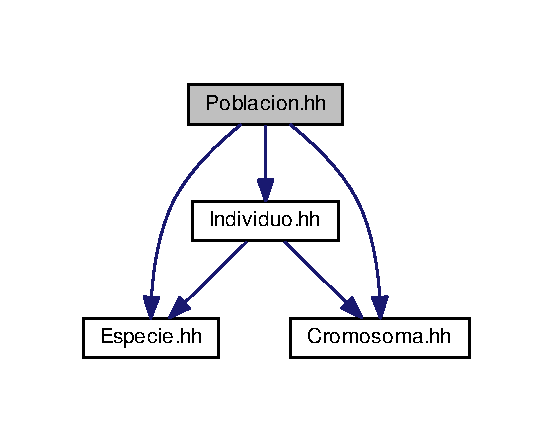
\includegraphics[width=266pt]{_poblacion_8hh__incl}
\end{center}
\end{figure}
\subsection*{Clases}
\begin{DoxyCompactItemize}
\item 
class \hyperlink{class_poblacion}{Poblacion}
\begin{DoxyCompactList}\small\item\em Representa un poblacion de individuos de una misma especie. \end{DoxyCompactList}\end{DoxyCompactItemize}


\subsection{Descripción detallada}
Especificación de la clase \hyperlink{class_poblacion}{Poblacion}. 


\hypertarget{pro2_8cc}{}\section{Referencia del Archivo pro2.\+cc}
\label{pro2_8cc}\index{pro2.\+cc@{pro2.\+cc}}


Programa principal para la práctica de P\+R\+O2\+: {\itshape Experimentos genéticos de laboratorio}.  


Dependencia gráfica adjunta para pro2.\+cc\+:\nopagebreak
\begin{figure}[H]
\begin{center}
\leavevmode
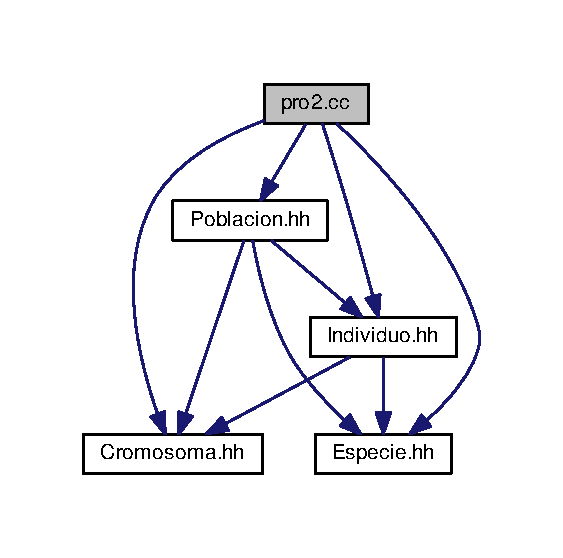
\includegraphics[width=270pt]{pro2_8cc__incl}
\end{center}
\end{figure}
\subsection*{Funciones}
\begin{DoxyCompactItemize}
\item 
int \hyperlink{pro2_8cc_ae66f6b31b5ad750f1fe042a706a4e3d4}{main} ()
\end{DoxyCompactItemize}


\subsection{Descripción detallada}
Programa principal para la práctica de P\+R\+O2\+: {\itshape Experimentos genéticos de laboratorio}. 



\subsection{Documentación de las funciones}
\index{pro2.\+cc@{pro2.\+cc}!main@{main}}
\index{main@{main}!pro2.\+cc@{pro2.\+cc}}
\subsubsection[{\texorpdfstring{main()}{main()}}]{\setlength{\rightskip}{0pt plus 5cm}int main (
\begin{DoxyParamCaption}
{}
\end{DoxyParamCaption}
)}\hypertarget{pro2_8cc_ae66f6b31b5ad750f1fe042a706a4e3d4}{}\label{pro2_8cc_ae66f6b31b5ad750f1fe042a706a4e3d4}


Definición en la línea 29 del archivo pro2.\+cc.


\begin{DoxyCode}
29            \{
30   \textcolor{comment}{// Inicialitzar}
31   \hyperlink{class_especie}{Especie}(esp);
32   esp.leer();
33 
34   \hyperlink{class_poblacion}{Poblacion}(pob);
35   pob.leer(esp);
36 
37   \textcolor{keywordtype}{string} s;
38   \textcolor{keywordflow}{while} (cin >> s and s != \textcolor{stringliteral}{"acabar"}) \{
39     \textcolor{comment}{// Añadir individuo}
40     \textcolor{keywordflow}{if} (s == \textcolor{stringliteral}{"anadir\_individuo"}) \{
41       \hyperlink{class_individuo}{Individuo}(ind);
42       ind.leer(esp);
43       cout << \textcolor{stringliteral}{"anadir\_individuo "} << ind.consultar\_nombre() << endl;
44       pob.anadir\_individuo(ind);
45     \}
46 
47     \textcolor{comment}{// Reproducir individuos}
48     \textcolor{keywordflow}{else} \textcolor{keywordflow}{if} (s == \textcolor{stringliteral}{"reproduccion\_sexual"})\{
49       \textcolor{keywordtype}{int} N = esp.consultar\_pares\_cromosomas();
50       vector<vector<int> > mat\_rep (N+1, vector<int> (3));
51       \textcolor{keywordtype}{string} madre, padre, hijo;
52       cin >> madre >> padre >> hijo;
53       \textcolor{keywordflow}{for}(\textcolor{keywordtype}{int} i = 0; i < N+1; ++i)\{
54         \textcolor{keywordflow}{for}(\textcolor{keywordtype}{int} j = 0; j < 3; ++j) cin >> mat\_rep[i][j];
55       \}
56       cout << \textcolor{stringliteral}{"reproduccion\_sexual "} << madre << \textcolor{charliteral}{' '} << padre << \textcolor{charliteral}{' '} << hijo << endl;
57       pob.reproducir(madre, padre, hijo, mat\_rep, esp);
58     \}
59 
60     \textcolor{comment}{// Escribir arbol de un individuo}
61     \textcolor{keywordflow}{else} \textcolor{keywordflow}{if} (s == \textcolor{stringliteral}{"escribir\_arbol\_genealogico"})\{
62       \textcolor{keywordtype}{string} ind; cin >> ind;
63       cout << \textcolor{stringliteral}{"escribir\_arbol\_genealogico "} << ind << endl;
64       pob.escribir\_arbol(ind);
65     \}
66 
67     \textcolor{comment}{// Completar arbol genealogico}
68     \textcolor{keywordflow}{else} \textcolor{keywordflow}{if} (s == \textcolor{stringliteral}{"completar\_arbol\_genealogico"})\{
69       queue<string> q;
70       \textcolor{keywordtype}{string} ind;
71       \textcolor{keywordflow}{while}(cin >> ind) q.push(ind);
72 
73       cout << \textcolor{stringliteral}{"completar\_arbol\_genealogico "} << q.front() << endl;
74       pob.completar\_arbol\_genealogico(q);
75     \}
76 
77     \textcolor{comment}{// Escribir poblacion}
78     \textcolor{keywordflow}{else} \textcolor{keywordflow}{if} (s == \textcolor{stringliteral}{"escribir\_poblacion"})\{
79       cout << \textcolor{stringliteral}{"escribir\_poblacion"} << endl;
80       pob.escribir();
81     \}
82 
83     \textcolor{comment}{// Escribir genotipo}
84     \textcolor{keywordflow}{else} \textcolor{keywordflow}{if} (s == \textcolor{stringliteral}{"escribir\_genotipo"})\{
85       \textcolor{keywordtype}{string} s; cin >> s;
86       cout << \textcolor{stringliteral}{"escribir\_genotipo "} << s << endl;
87       pob.escribir\_genotipo(s);
88     \}
89 
90     \textcolor{comment}{// Fin}
91     \textcolor{keywordflow}{else} \{
92       \textcolor{keywordflow}{return} 0;
93     \}
94   \}
95 
96 \}
\end{DoxyCode}

%--- End generated contents ---

% Index
\backmatter
\newpage
\phantomsection
\clearemptydoublepage
\addcontentsline{toc}{chapter}{Índice}
\printindex

\end{document}
